\graphicspath{ {./images/} }
\chapter{背景與相關研究}
\label{c:background}


\section{區塊鏈}

在區塊鏈網路中的每一個全節點(full node)都會維護一份完整的賬本,
賬本記錄了過往所有區塊中的交易,由此我們能夠知曉交易發生的時間點、交易的付款人收款人、交易的金額,
付款人得以向付款人證明自己確實已經付款。

區塊鏈網路中,賬本的更新以區塊為單位,
當一個礦工節點蒐集交易並挖掘出一個區塊後,
會將它廣播到網路上,收到區塊的節點必須驗證後決定是否接收,
若接收,賬本的內容就得到更新。

根據收付款的方式, 區塊鏈貨幣可分為類似銀行賬戶式的賬戶系統,
以及類似零錢式的 UTXO (unspent transaction output) 系統。

賬戶系統中,每個用戶擁有一個地址,地址有它相對應的私鑰,
經由私鑰簽章,用戶就能將他持有的資產轉移到其他地址。

UTXO 系統中存在著大量的 UTXO ,每個 UTXO 上有一個腳本,
當一個使用者能夠提供一個輸入(通常是使用他的私鑰簽名)使得腳本執行結果為真,
他就得以花費這筆 UTXO ,花費 UTXO 後會產生其他的 UTXO ,
只要新生成的 UTXO 只有收款人才能花費,資產的轉移就完成了。
在 UTXO 系統中,使用者擁有的是一組它能夠花費的 UTXO ,
而非一個賬戶上的一個代表存款的數字。

在本論文中,只關注基於賬戶的區塊鏈系統,忽略 UTXO 的區塊鏈系統。

\subsection{區塊驗證}

在支援智慧合約的賬戶系統中,對於區塊中的一般交易,
節點必須知道付款人是否有足夠的餘額;
若涉及智慧合約,節點需要獲取合約程式碼以及合約當前的狀態,
才能夠執行合約。

我們可以用一個鍵值對來表示賬戶系統在驗證交易時所需要儲存的資訊:

\[state = f: address\to account \]

給一個地址,我們能得到對應賬戶的資訊,可能是餘額,也可能是智慧合約的狀態。

若要儘速完成這些工作,節點必須快速地檢索交易,因此,
一個一個區塊地尋找、計算出賬戶資訊是不切實際的, 
通常節點會內置一個資料庫,並利用資料庫的索引來高速完成查詢工作。

\subsection{狀態儲存的問題}

區塊鏈的狀態儲存方式造成了兩個衝擊:

\begin{enumerate}
  \item 佔用儲存空間大
  \item 驗證交易時需要資料儲存裝置的隨機存取
\end{enumerate}

\subsubsection{佔用儲存空間大}

永遠增長的區塊已經對節點維護者造成負擔,比特幣與以太坊佔用的空間都已經超過 200 GB ,
如果在 AWS 上租用機器來運行以太坊節點,每個月需花費 50 - 70 美金,
這個成本如果降不下來,慈善節點的數量勢必會不斷下滑,
根據 \href{https://web.archive.org}{Wayback Machine} 上 \url{https://ethernodes.org/} 的資訊,
\href{https://web.archive.org/web/20180224224831/https://www.ethernodes.org/network/1}{2018 年 2 月}有逾兩萬個節點,
\href{https://web.archive.org/web/20200512075927/https://www.ethernodes.org/}{2020 年 5 月}已經下降到七千。

另外一個問題是,以太坊中存在許多智慧合約已經不再被使用,例如 EOS 的 首次貨幣發行 (ICO) ,
在發行結束後,該合約已無作用,但所有的全節點卻仍得繼續儲存它的歷史數據。
這類僅有短暫效力的合約這無疑造成了大量的空間浪費。

\subsubsection{需要資料儲存裝置隨機存取}
交易中的賬戶地址沒有規則,因此當節點驗證交易,去獲取賬戶狀態時,
必須進行隨機存取,一個區塊中有幾筆交易,就必須進行幾次隨機存取。
傳統硬碟的存取依賴讀寫頭移動跟碟片旋轉,隨機操作的效率低下,
以致於使用傳統硬碟的節點甚至無法跟上以太坊網路 15 TPS (transaction per second) 的交易速度。
不得不使用造價較為昂貴的固態硬碟又進一步加劇了節點維護者的經濟負擔。

\section{無狀態區塊鏈}
為了解決上述問題,區塊鏈社群提出了狀態租賃(state rent)、
狀態修剪(state pruning)、無狀態區塊鏈(stateless blockchain)等等改進方案。

以下介紹無狀態區塊鏈的概念。

無狀態區塊鏈的核心想法在於,節點能否在只儲存區塊標頭的情況下,
仍然能夠驗證交易的正確性?

可以的,如果我們在交易中附上一些額外資訊,並且以區塊標頭來驗證這些額外資訊無誤,
就能夠利用這些額外資訊來驗證交易的正確性了。

在賬戶系統中,則可以讓所有賬戶狀態構成一顆梅克爾 Patricia 樹(patricia merkle tree)
或是稀疏梅克爾樹(sparse merkle tree)\cite{dahlberg2016efficient},
並且在區塊標頭裡放入根(也就是整個狀態的摘要),
在交易中附上付款人的餘額,以及付款人狀態的梅克爾路徑(merkle path),
如此,就可以確認付款人的餘額,再去看它是否足夠支應本次交易。

圖 2.1 是一般區塊鏈交易與無狀態區塊鏈交易的對比,
同樣是一筆 Bob 給 Alice 200 元的交易,在無狀態區塊鏈上,
必須多附上一筆證明(黃色部分),以供無狀態節點驗證交易的合法性。

\begin{figure}
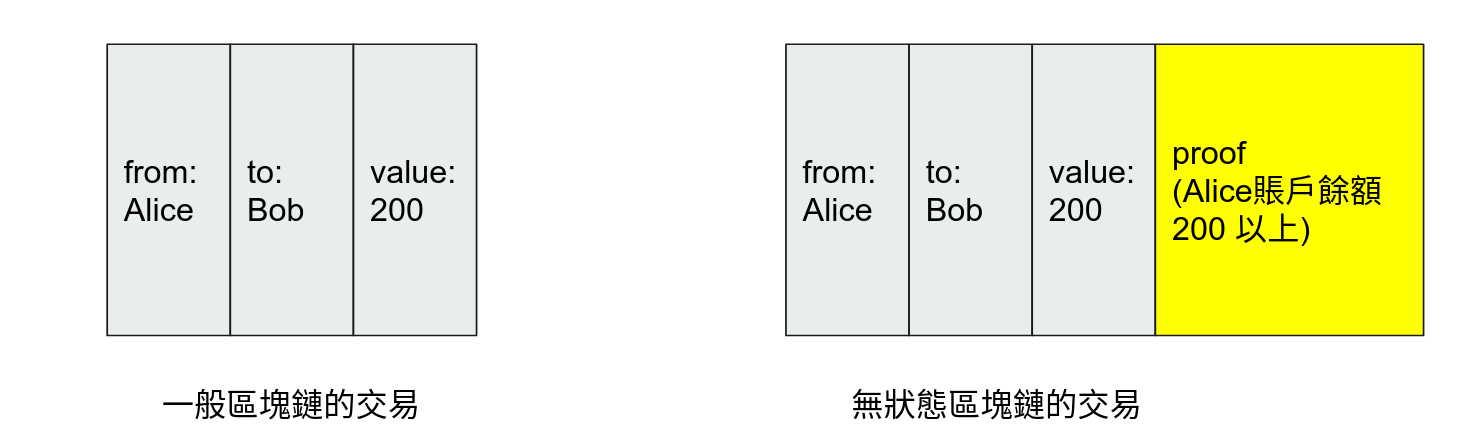
\includegraphics[width=\textwidth]{stateless-tx}
\caption{一般區塊鏈、無狀態區塊鏈交易比較}
\end{figure}

\subsection{vector commitment}

不僅僅上述的梅克爾樹變形能夠生成、更新摘要和證明,
可以做到這些功能的結構被稱為 vector commitment\cite{catalano2013vector}。

近年來, vector commitment 領域也持續出現不同針對無狀態區塊鏈的代數構造,
它們相較於梅克爾樹,時空間複雜度更小,或是擁有其他優點:
有的能夠將多個證明打包以降低空間\cite{boneh2019batching},
有的則有同態加法的特性,使得製作交易證明時,付款人不用知道收款人的當前餘額\cite{chepurnoy2018edrax}。

\section{快取證明}

Utreexo~\cite{dryja2019utreexo} 應用梅克爾樹構成的森林設計了一種新的 accumulator ~\cite{benaloh1993one},
基於此種 accumulator ,Utreexo 節點不需要真正的儲存比特幣所有的 UTXO ,
就能夠驗證區塊。

該篇論文也提及到,分析比特幣的歷史記錄,
約有 40\% 的 UTXO 會在 20 個區塊內被消耗,
將近 80\% 的 UTXO 會在 1000 個區塊內被消耗,
因此使用少量的記憶體空間來快取最近出現的 UTXO ,就能夠省略傳輸許多證明。

然而, Utreexo 僅僅討論了在初始同步節點資料時的情形,
並未考慮到同步到最長鏈之後可能發生的分叉問題。此外,
由於 UTXO 的產生與消耗都各只有一次,
使得具有統計性質的快取策略難以應用,而在賬戶系統中,
賬戶可以多次出現,因此可以應用的快取策略更廣泛。

本論文將會討論在賬戶系統中該如何應對分叉問題,
以及 LRU 快取策略在賬戶系統中的使用。

\subsection{持久化資料結構}

為了在分叉情況下高效存取快取,我們將會使用持久化資料結構,
故先行在此介紹基本概念與相關技巧。

如果一種資料結構在修改之後,能夠保留之前的版本,
就可以被稱為持久化資料結構\cite{driscoll1986making}(Persistent Data Structure),
與之相對的是暫時性資料結構(Ephemeral Data Structure)。

\subsubsection{路徑複製}
對於樹這種資料結構,可以利用路徑複製的技巧來將它變得持久化,
當樹中的一個節點被修改,就連帶修改指向它的父親節點,
如此一直遞迴往上修改到根節點,就可以得到一棵新版本的樹。

\begin{figure}
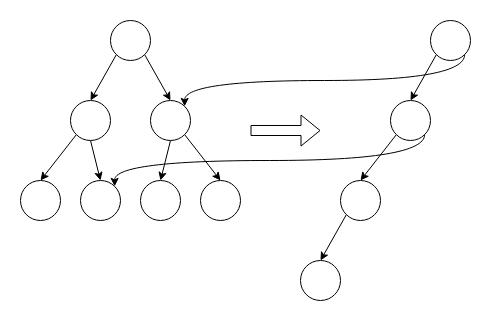
\includegraphics[width=\textwidth]{../images/路徑複製.png}
\caption{路徑複製}
\end{figure}

圖 2.2 是一個路徑複製的例子,可以從圖中看到,
只有被插入葉子的節點所在的分支被複製了一趟。
